\documentclass[12pt, a4paper]{article}
\usepackage[utf8]{inputenc}
\usepackage{geometry}
\usepackage{titlesec, hyperref, bbm}
\usepackage{amsmath, amssymb}
\usepackage{graphicx}
\usepackage{indentfirst}
\usepackage[english]{babel}

\hypersetup{
    colorlinks,
    citecolor=black,
    linkcolor=black,
    urlcolor=black,
}

\title{Intraday Value at Risk (IVaR) Using Tick-by-Tick Data with Application to the Toronto Stock Exchange}
\author{Peng-Wei Chen}
\date{March 2022}

\begin{document}
\maketitle

\section{Original article}
We first give an overview of the original article \cite{Toronto}.
\subsection{Objectif}
\par
The Value at Risk (VaR) is the maximum expected loss at a given confidence level.
Banks and institutions often generate the VaR at the end of  day in order to determine their risk exposure.
The VaR calculated is thus the base of their risk measurement.
However, due to the popularization of the electronic trading, more and more data are produced,
and the old measure method is no longer adequate.
Moreover, the old method also takes so much time since these financial institutions have a lot of products/services at the same time,
and the method was based on a great number of Monte-Carlo simulation.
\par
The proposal of Intraday Value at Risk (IVaR) was to improve the use of  the daily trade data, 
and to get an accurate VaR using it.
Comparing to VaR which is at a higher timeframe (~10 days) and with a more discrete price, 
the IVaR can be provided at during the daily trade.

\subsection{Model description}
The model first uses log-Autoregressive Conditional Duration (log-ACD) model to handle the irregular timestamp difference.
After that, they use the ultra-high-frequency (UHF) GARCH model for the price return,
divided by a function of duration for the normalization.
Once the parameters are determined, 
the IVaR is then calculated with a Monte Carlo simulation.

\subsubsection{Background}
Consider a series of trades $(t_i)_{i\in \mathbb{N}}$, where we have the corresponding prices $(p_i)_{i\in \mathbb{N}}$.
Let the process $(x_i)_{i\in\mathbb{N}}$ be the duration between $i^{th}$ and $(i+1)^{th}$
and the return process $(r_i)_{i\in\mathbb{N}}$ defined by $r_i = \log (\frac{p_i}{p_{i-1}})$.
Then the transaction process can be written by 
$$\{ (x_i, r_i), i\in \mathbb{N}\}$$
The idea is to define the low of $(x_i, r_i)$ on the past filtration $\mathcal{F}_{i-1}$.
$$(x_i, r_i) | \mathcal{F}_{i-1} \sim f\left( x_i, r_i | \overline{x_{i-1}}, \overline{r_{i-1}}; \theta \right)$$
where $\overline{s_{i}} = (s_j)_{j \le i}$ is the past events.
We can rewrite the density function $f$ to the following one:
$$f\left( x_i, r_i|\overline{x_{i-1}}, \overline{r_{i-1}}; \theta \right) = g\left( x_i|\overline{x_{i-1}}, \overline{r_{i-1}}; \theta_1 \right)q\left( r_i|x_i, \overline{x_{i-1}}, \overline{r_{i-1}}; \theta_2 \right)$$
$g$ is the low of the new duration based on past information and $q$ is the conditional low knowing past information and the new duration. 

Finally, we maximize the log likelihood
\begin{equation}
\mathcal{L}(\theta_1, \theta_2) = \sum_{i=1}^n \left[ \log g(x_i|\overline{x_{i-1}}, \overline{r_{i-1}}; \theta_1) + \log q(r_i|x_i, \overline{x_{i-1}}, \overline{r_{i-1}}; \theta_2) \right]
\label{max_likelihood}
\end{equation}
Note that we maximize $\theta_1, \theta_2$ at the sametime.

In order to calculate the IVaR, we then use the Monte Carlo method with the above models.
\subsubsection{ACD model}
In the ACD model, we estimated the conditional duration $\psi_i$ by
$$\psi_i = \mathbb{E}(x_i|\mathcal{F}_{i-1}) \ge 0$$
In the assumption of the ACD model, we suppose that the ratio $\frac{x_i}{\psi_i}$ is independent and identically distributed (i.i.d.)
$$x_i = \psi_i \varepsilon_i$$
Where $\varepsilon_i$ should be non-negative and $\mathbb{E}(\varepsilon_i) = 1$. 

We can then for example define the function of $\psi_i$ by whether
$$\psi_i = \omega + \sum_{j=1}^m \alpha_j x_{i-j} + \sum_{j=1}^q \beta_j \psi_{i-j}$$
for the normal ACD$(m, q)$ model or
\begin{equation}
\psi_i = \exp\left( \omega + \sum_{j=1}^m \alpha_j \varepsilon_{i-j} + \sum_{j=1}^q \beta_j ln(\psi_{i-j})\right)
\end{equation}
for the log-ACD model. Where $\omega, \alpha_i, i\in{[1, m]}, \beta_j, j\in{[1, q]}$ are positive.


\subsubsection{UHF-GARCH model}
The GARCH model proposed by Engle (2000) is used in their article to simulate the conditional variance per transaction:
$$h_i = V(r_i|\overline{x_i}, \overline{r_{i-1}})$$
which is the expected variance at the $i^{th}$ transaction, conditional on the past information.
Note that $h_i$ is the variance with respect to the duration:
$$h_i = x_i \sigma^2_i$$
and we modeled it with a simple GARCH(1, 1) (under assumption that $\mathbb{E}(r_i|\overline{x_i}, \overline{r_{i-1}}) = 0$):
$$\sigma^2_i = \tilde{\omega} + \tilde{\alpha}\left( \frac{r_{i-1}}{\sqrt{x_{i-1}}} \right)^2 + \tilde{\beta} \sigma^2_{i-1}$$
where $\tilde{\omega} > 0, \tilde{\alpha}\ge 0$ and $\tilde{\beta} \ge 0$.

\subsubsection{Monte Carlo IVaR}
The idea is simple. As shown in Figure \ref{fig:monte_carlo}, we fix a time interval to T units of time and a number $P$ for the number of units. We then start simulating the process with the log-ACD(1,1) and the UHF-GARCH models. Once the duration exceeds $PT$, we have thus obtained $P$ samples of trade transactions:

The IVaR at $k$ units of time $\mbox{IVaR}_k$ with confidence level $1 - \alpha$ is defined as
$$\mathbb{P}\left( y_k < -\mbox{IVaR}_k(\alpha) | \mathcal{G}_k \right) = \alpha$$

\begin{figure}
    \centering
    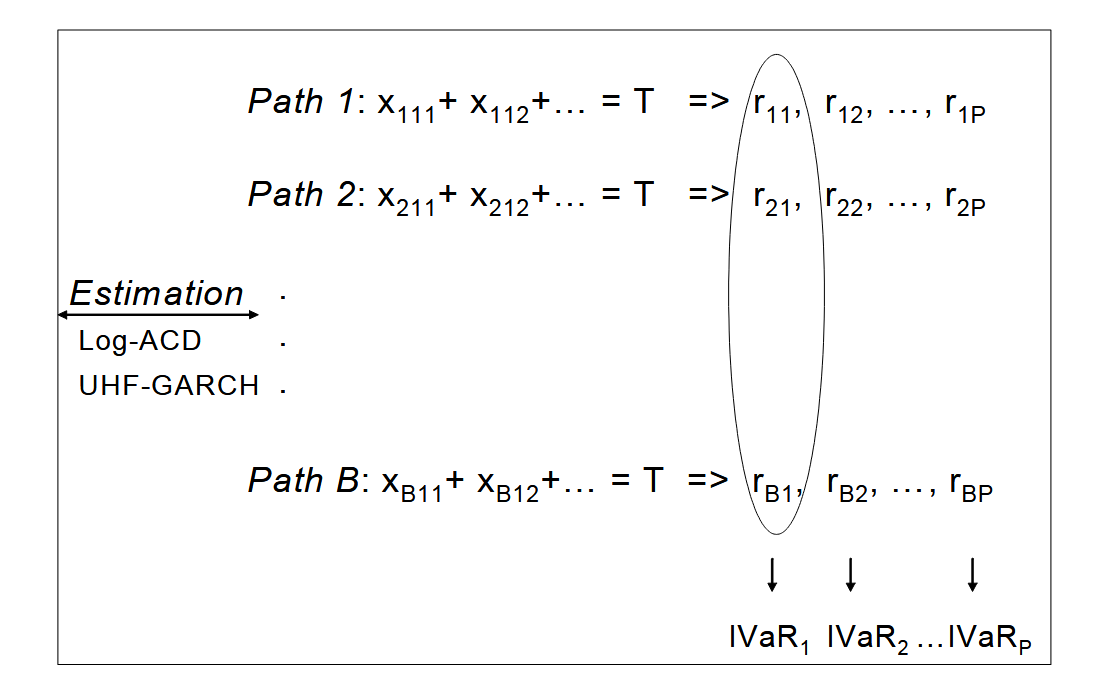
\includegraphics[scale=0.4]{MonteCarlo.png}
    \caption{How we calculate the IVaR with the Monte Carlo method. Note that for each path, the series of $x_{i,j,k}$ ends with $x_{i,P,-}$ where P is the number of intervals that we want to calculate the IVaR. Source : \cite{Toronto}}
    \label{fig:monte_carlo}
\end{figure}

\subsubsection{Extended UHF-GARCH model}
Instead of the UHF-GARCH, we propose the extended one, where $h_i$ is not directly related to the duration:
$$h_i = x_i^\gamma\sigma_i^2$$
At the same time, we use the ARMA(1,1) model on the tick-by-tick returns:
$$r_i = c + \phi_1 r_{i-1} + e_i + \theta_1 e_{i-1}$$
$c, \phi_1, \theta_1$ are constants. In this case, the GARCH can be written as:
$$\log \sigma^2_i = \tilde{\omega} + \sum_{j=1}^P \tilde{\beta_j} \log \sigma^2_{i-j} + \sum_{j=1}^Q a_j  \left\{ \frac{|e_{i-j}|}{\sqrt{h_{i-j}}} - \mathbb{E}\left( \frac{|e_{i-j}|}{\sqrt{h_{i-j}}} \right) \right\} + \sum_{j=1}^{Q} \tilde{\alpha_j}\left( \frac{e_{i-j}}{\sqrt{h_{i-j}}} \right)$$
where $e_i = z_i \sqrt{h_i}$ and $z = \{ z_i, i \in \mathbb{Z}\}$ are a strong white noise with zero mean and unit variance and $\tilde{\omega}, \tilde{\beta_j}, a_j$ and $\tilde{\alpha_j}$ are constants $\ge 0$.

\subsection{Numerical result}
The model was tested on the Royal Bank  of Canada stock (RY) and the Placer Dome stock (PDG) on the Toronto Stock Exchange (TSE). Regular trading starts at 9:30 and ends at 16:00. The transaction prices are used for the calculation of return. This is because when we want to liquidate positions, one has to transact either on the ask or the bid. Therefore, using the midquote-change quantiles may underestimate the true VaR.

We first clean up the data with duration larger than 25 standard deviations, and 10 standard deviations for the absolute returns. This results in a number of 51,660 observations for the RY stock and 27,956 observations for the PDG stock.
\subsubsection{Seasonal data adjustment}
In order to have a more generalized result, we make some adjustment to the data due to the seasonality. It includes:
\begin{itemize}
    \item Interday effects ($\bar{u_s}$ means the average value of $u$ for day s):
    \begin{itemize}
        \item $x_{t, inter} = \frac{x_t}{\bar{x_s}}$
        \item $r_{t, inter} = \frac{r_t}{\sqrt{\bar{r^2_s}}}$
    \end{itemize}
    \item Once identified, we remove the intraday effects by (The expectation is calculated by averaging the variables over thirty minutes intervals for each day of the week, then  using cubic splines on these intervals)
    \begin{itemize}
        \item $x_{t, intra} = \frac{x_{t, inter}}{E(x_{t, inter} | \mathcal{F}_{t-1})}$
        \item $r_{t, intra} = \frac{r_{t, inter}}{\sqrt{E(r^2_{t, inter} | \mathcal{F}_{t-1})}}$
    \end{itemize}
\end{itemize}
The de-seasonality effect needs to be considered: by setting a dummy variables to each day of the week, the coefficients for the regression rejects the null hypothesis of equality of them with a Wald test. The results of intraday seasonal effects on RY for durations and squared returns are shown in Figure \ref{fig:durations} and Figure \ref{fig:squared_returns}.
\begin{figure}[htpf!]
    \centering
    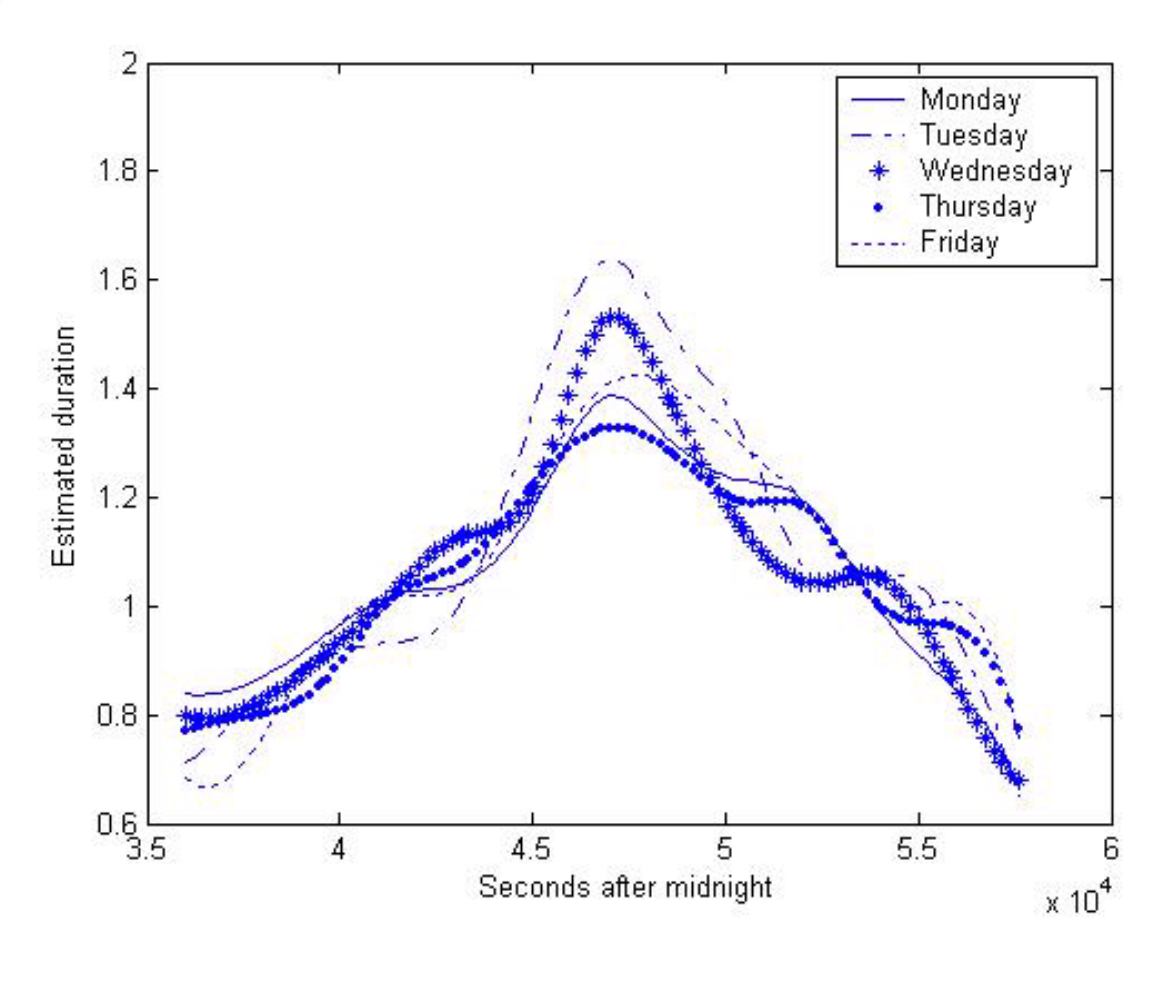
\includegraphics[scale=0.3]{Seasonality.png}
    \caption{Intraday seasonality for RY durations}
    \label{fig:durations}
\end{figure}

\begin{figure}
    \centering
    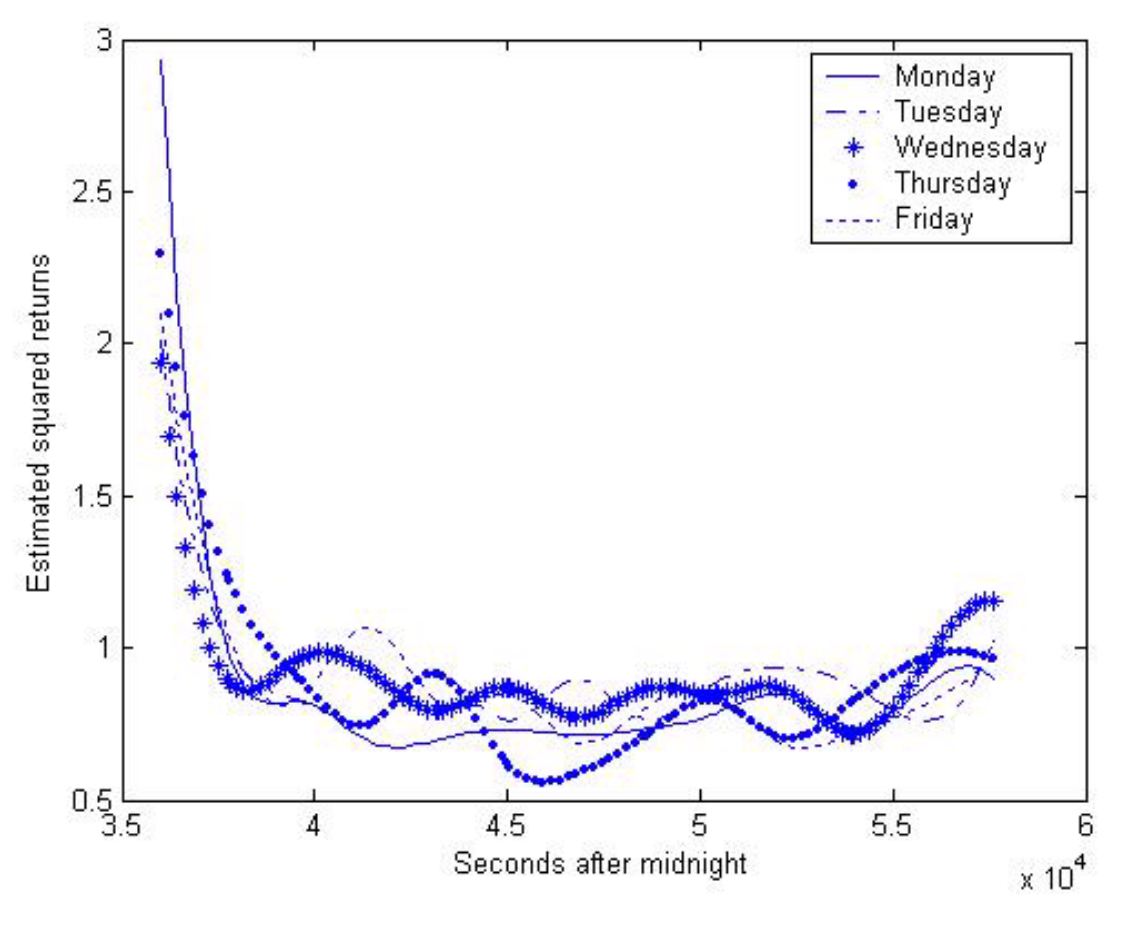
\includegraphics[scale=0.3]{IntradaySeasonality.png}
    \caption{Intraday seasonality for RY squared returns}
    \label{fig:squared_returns}
\end{figure}

\subsubsection{Estimation Results}
The model was trained on the first month of data,  while tested on the next two months of data. We first tested the auto-correlation effect with the Ljung-Box test Q(15). The usage of GARCH and ACD models is well justified with the high coefficients in returns and in duration, while the p-value rests higher than 0.05. Finally, we retain a log-GACD(2,2) model for the duration and a ARMA(1,1)-UHF-GARCH(1,1) model for the return (Figure \ref{fig:IVaR_coeff}).

\begin{figure}[htpf!]
    \centering
    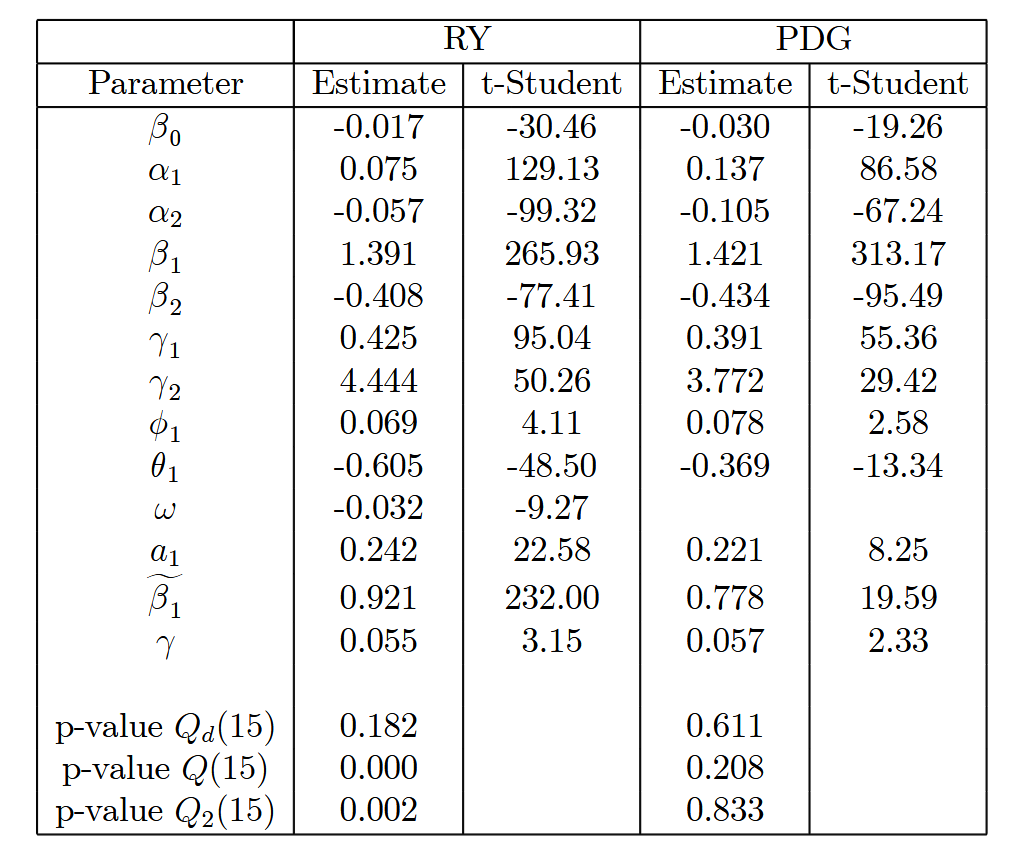
\includegraphics[scale=0.3]{Coefficients.png}
    \caption{The coefficients for log-ACD-UHF-GARCH model.}
    \label{fig:IVaR_coeff}
\end{figure}

The performance was quantified with the Kupiec's test. We first compute the empirical failure rate $\hat{\alpha}$ with the historical data. We propose the null hypothesis $\hat{\alpha} = \alpha$. We then consider the Kupiec's likelihood ratio
$$
LR = 2[\ln(\hat{\alpha}^m(1-\hat{\alpha}^{n-m}) - \ln(\alpha^m(1-\alpha)^{n-m})]
$$
where $m$ is the number of exceptions and $n$ is the sample size. $LR$ is asymptotically distributed as a $\chi^2(1)$ under the null hypothesis. The model was rejected only with some short interval and high VaR levels. While the interval length is too small, we have less chances to get non-zero returns and thus the violations  of IVaR cannot be achieved.

Another test of dynamic quantile (DQ) proposed by Engle and Manganelli was also used to check the IVaR's property. In fact, the violations should not be correlated serially. We define thus
$$
Hit_k = I(y_k  < -IVaR_k) - \alpha
$$
The DQ test consists of modeling the variable $Hit_k$ by a linear regression $Hit_k = XB + \epsilon_k$. Then we get a Wald-like statistic $DQ=\frac{\hat{B'}X'X\hat{B}}{(\alpha(1-\alpha))} \sim \chi^2(l)$ where $l$ is the number of explanatory variables and $\hat{B}$ is the OLS estimate ofo B. In most of the cases, we get a p-values greater than 0.05.


\begin{figure}[htpf!]
    \centering
    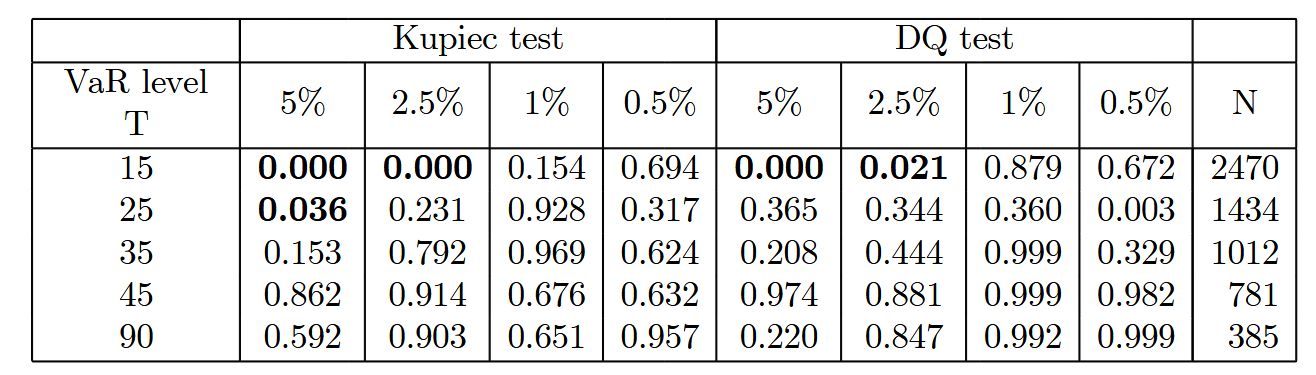
\includegraphics[scale=0.3]{IVaR results RY.png}
    \caption{The Kupiec's and DQ test on RY.}
    \label{fig:IVaR_results_RY}
\end{figure}

\begin{figure}[htpf!]
    \centering
    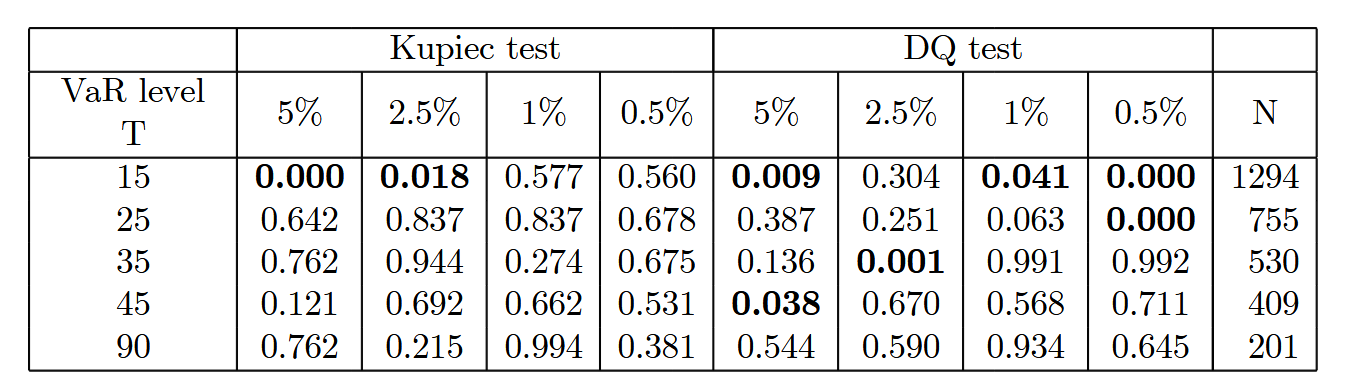
\includegraphics[scale=0.3]{IVaR results PDG.png}
    \caption{The Kupiec's and DQ test on PDG.}
    \label{fig:IVaR_results_PDG}
\end{figure}

Finally, we give an illustration of the calculated IVaR value with the Monte Carlo method in Figure \ref{fig:IVaR}.

\begin{figure}[htpf!]
    \centering
    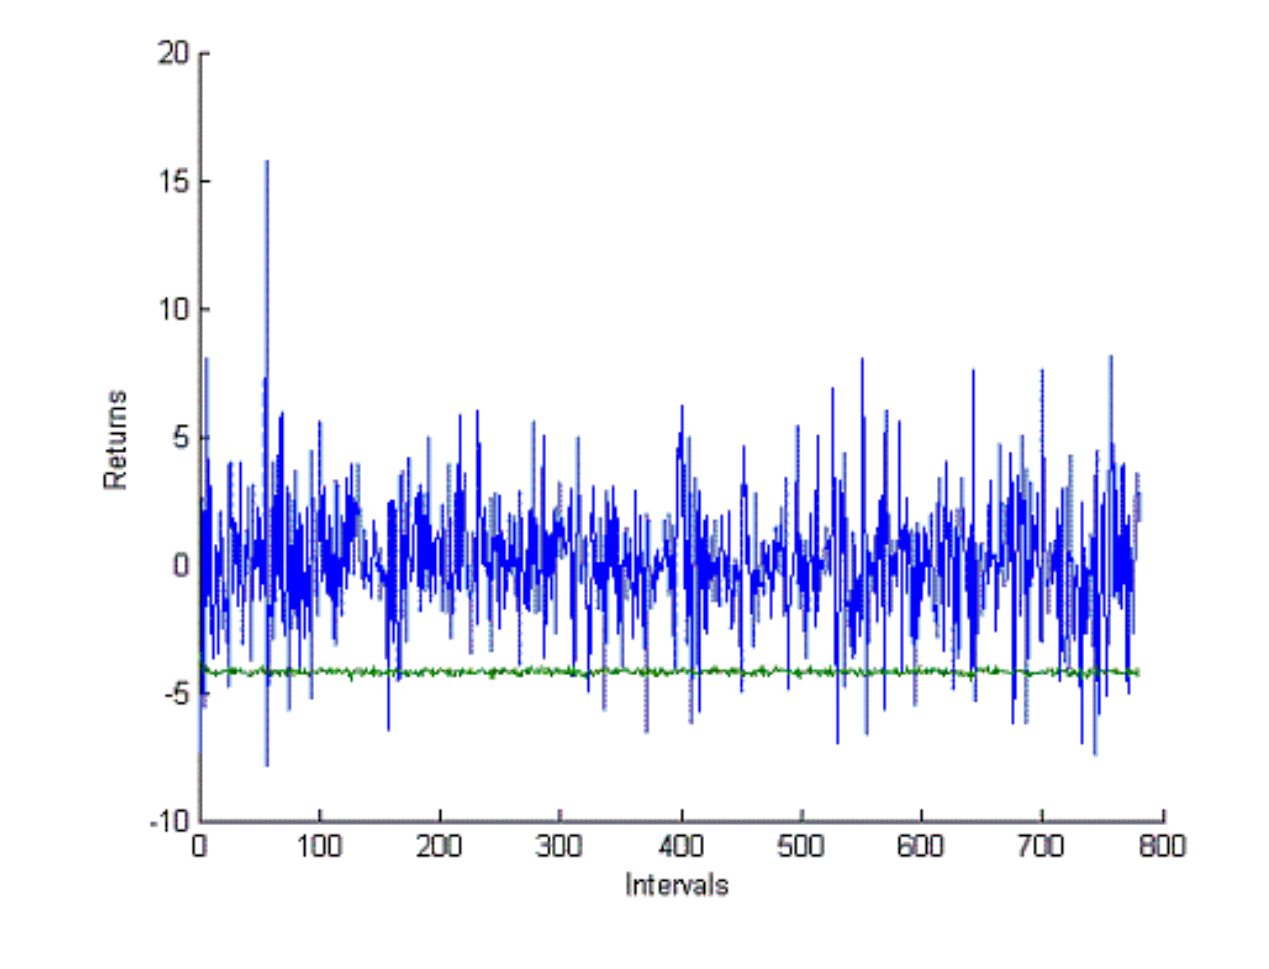
\includegraphics[scale=0.3]{Result_IVaR}
    \caption{The Monte Carlo obtained IVaR value (green line) with respect to the returns series.}
    \label{fig:IVaR}
\end{figure}
\subsubsection{Conclusion of the original article}
Applying the log-GACD(2,2)-ARMA(1,1)-UHF-GARCH(1,1) model and the Monte Carlo simulation, we arrive to forecast the returns for any arbitrary interval length. After the removal of the seasonality, the model performs well with historical data while the error term is supposed to be a normal distribution. We can thus define the IVaR on tick-by-tick data.

\section{Personnel criticism and bibliography}
\subsection{Personnel criticism}
\subsubsection{Data frequency}
The approach here is so old to be useful: in fact, the data set they used dated from April 1st to June 30, 2001. This is when the high frequency trading began to emerge. But the frequency is still at "mid-frequency" level from today's point of view: the average of duration between two trades is around 30 seconds and 1 minute in their data. This means that the market is not as efficient as we are today, taking the US stock markets for example. As for today's usage, one might also notice that if we want to calculate $\mbox{IVaR}_k(\alpha)$ with their Monte-Carlo method, we will need much more calculations since the average duration is much smaller. This should also be taken into concern in practice.

\subsubsection{Numerical result}
A critical problem in their numerical result is that their result doesn't verify the assumption. Indeed, we assumed that the coefficients are positive for the ACD and the GARCH models. However, we can clearly see the negative estimations in their results in spite of their good p-values. The result is more "locally" correct for me and it can not handle the extreme outliers. One should review this point before practicing the IVaR calculation.

\subsubsection{Maximum likelihood}
In (\ref{max_likelihood}), we try to maximize the log likelihood on both ACD and Extended UHF-GARCH model at the same time. Although it is much more complicated to do so, it can be explained by the fact that the duration and the return can not be treated separately. This is shown in \cite{dur_return} on NYSE stocks, given by the original article.

However, we have to mention that in \cite{dur_return}, the week exogeneity was shown using the exponential, Gaussian and Poisson distribution. This is incoherent to the generalized gamma distribution used in the work. We are not sure if we can still reject the null hypothesis with the generalized gamma distribution.

\subsection{Bibliography}
\subsubsection{ACD model}
The ACD model was first introduced in \cite{ACD} in order to model the duration between trading events. Dated from 1998, we might investigate more on its utility nowadays.

It could explain the clustering of the transactions. In fact, we can observe that most of the transactions are clustered with others transactions at some moments. It did share a lots of features with the GARCH model since they are used to model the autoregressive parts in financial data. The ACD model is still in studies in the past few years with different varieties and tested on different data set, such as \cite{acd_NYSE}, \cite{nonstationary_acd}.

In \cite{acd_NYSE}, the author apply the ACD model on the SPY duration from 01/02/2014 to 12/31/2014. He compares the Exponential, Weibull, Gamma and Generalized Pareto distributions. After the removal of intraday seasonality, the simple ACD (without log variance) model can well describe the SPY duration with a Gamma distribution. This shows that even with a supposed more efficient market (the American index in 2014), the ACD model can still be a good proxy to model the duration.

In \cite{nonstationary_acd}, the authors propose a time varying-ACD (tv-ACD) model by setting the parameters as a function of time. We define the tv-ACD(1, 1) model for a process by
$$
x_i = \psi_i\epsilon_i,
$$
$$
\psi_i = \omega(i) + \alpha(i)x_{i-1} + \beta(i)\psi_{i-1}
$$
where $\omega(\cdot), \alpha(\cdot), \beta(\cdot)$ are non-negative functions. It can be proved that we can approximate the functions with a polynomial approach.

There are still a lot of variants of ACD model as cited in \cite{nonstationary_acd}. We provide some of them (in (1, 1) form) as follows:
\begin{itemize}
    \item Log-ACD1$(1,1)$: $\ln \psi_i = \omega + \alpha \ln \epsilon_{i-1} + \beta \ln \psi_{i-1} $
    \item Log-ACD2$(1,1)$: $\ln \psi_i = \omega + \alpha \epsilon_{i-1} + \beta \ln \psi_{i-1} $
    \item AMACD$(1,1,1)$: $\psi_i = \omega + \alpha x_{i-1} + \nu \epsilon_{i-1} + \beta \psi_{i-1} $
    \item ABACD$(1,1)$: $\psi_i^{\delta_1} = \omega + \alpha(|\epsilon_{i-1} - \nu| + c|\epsilon_{i-1} - \nu|)^{\delta_2} + \beta \psi_{i-1}^{\delta_1}$
\end{itemize}

\subsubsection{UHF-GARCH model for returns}
The UHF-GARCH model is an application of the ACD model. It needs to be applied with the ACD model since the return rate depends on the last duration. The maximum-likelihood method is then applied in order to determinate different parameters in common approach. Recent research uses the UHF-GARCH model mostly to forecast the volatility and for the pricing usage, combining with the Monte Carlo method. There is an article \cite{forecasting} discussing if the duration model really matters in the UHF-GARCH model. In \cite{vol}, one discusses the comparison within the integrated volatility and the UHF-GARCH model.

In \cite{forecasting}, the authors test the UHF-GARCH model with a Weibull-ACD, Exponential ACD and the Burr-ACD modle, with the GMM (Generalized method of moments) estimation of the duration model and the Maximum Likelihood approach for the volatility forecast. The difference consists of using different distributions for the error term in the ACD model. In the end, we show that on the German stock market data, the Exponential distribution produces an instable result, whereas the Weibull one is rather robust and the result with Burr distribution didn't give more improvement to the Weibull one. This shows that the generalized gamma distribution could be a good choice while the Weibull distribution belongs to it.

The integrated volatility is measured by the squared value of intradaily returns $\sigma^2_I(m) = \frac{1}{n}\sum^N_{n=1} r^2_{m,n}$ for the nth squared return on day $m$. In \cite{vol}, they forecast the volatility in n units of time using a GARCH(1,1) model on the integrated volatility, forecasting with ACD-UHF-GARCH model with ARMA(1,1) in return (same as the one in this article) and the integrated volatility method. Then we run the Mincer-Zarnowitz regression $y_t = c + \beta y_{ft} + \varepsilon_t$ where $c, \beta$ are constants, $\varepsilon_t$ is a white noise and $y_t$ means the price at time $t$. Finally, they test the coefficients with the t statistics.  They show that the integrated volatility and the UHF-GARCH model both lead to poor performances in volatility forecasting, while the integrated volatility has a greater performance.

This supposed that the Intraday VaR calculated might not be as good as we think.


\subsubsection{Intraday VaR calculations}
In \cite{Giot} (Access restricted for me), the author proposes uses regularly spaced intraday returns with the Gaussian GARCH and t-GARCH model for the calibration. This method was then reused in the article \cite{asym-ACD}, in order to compare with the method in \cite{Toronto} and their proper method. Finally, they claim to outperform \cite{Toronto} by replacting the duration model by asymmetric autoregressive conditional duration (AACD) model. The method is mainly the same as the one in the original article, simply replacing the log-ACD model by the AACD model. We calibrate both models with the maximum likelihood method and then use the Monte Carlo to simulate the IVaR. There are still a lot of possibilities out there for the IVaR calculation.

%TODO

\section{Conclusion}
Different models are still under studying for the tick-by-tick data. The authors propose a way to simulate the price process with the duration and the price return. Under this simulation, we can do Monte Carlo simulations in order to find out the Value at Risk with intraday data. This is extremely useful since we won't need to wait until the end of day to calculate the VaR anymore.

However, more and more models are proposed in recent research and several tests might suggest that the usage of ACD-UHF-GARCH model isn't good enough for the Intraday VaR calculation. One might check the most recent results in order to update their models in practice.

\newpage
\bibliographystyle{plain}
\bibliography{references}
\end{document}
